\documentclass[lettersize,journal]{IEEEtran}
\usepackage[utf8]{inputenc}
\usepackage{outlines}
\usepackage{graphicx}
\usepackage[inline]{enumitem}
\usepackage{wrapfig}
\usepackage{makecell}
\usepackage{pifont}% http://ctan.org/pkg/pifont
\usepackage{amsthm}
\usepackage{amsmath}
\usepackage{mathtools}
%\usepackage{amssymb}
\usepackage{stmaryrd} % Additional math symbols.
\usepackage{amsfonts}
\usepackage{flushend}
\usepackage{balance}
%\usepackage[hyphens]{url}
\usepackage{hyperref}
\usepackage{multicol}
\usepackage{multirow}
\usepackage{setspace} % For double, 1.5, single spacing etc.
\usepackage{xspace}
\usepackage{listings}
\usepackage{ifthen}
\usepackage{verbatim}
\usepackage{float} % Defines newfloat used below
\usepackage{subcaption}
\usepackage{microtype}
\usepackage{mathptmx} % Fails the display of parentheses in math environment
\usepackage{textcomp}
%\usepackage[sort&compress]{natbib}
\usepackage{booktabs}
\usepackage{longtable}
\usepackage{blindtext}
\usepackage{fancyhdr}
%These two let you use multibyte utf-8 characters, e.g. 03bb - λ 
\usepackage[mathletters]{ucs}
\usepackage[utf8]{inputenc}
\usepackage{wasysym}	% Defines \cent, \currency, \brokenvert
\usepackage{tikz}
\usepackage{esvect}
\usepackage{csquotes}
\usepackage{array}
\usepackage{xcolor, colortbl}
\usepackage{tablefootnote}
\usepackage{supertabular}
% hyperref redefines a number of macros, so it should be last.  Empirically,
% doing so eliminates compiler warnings.
%\usepackage[bookmarks, colorlinks, citecolor=green, urlcolor=blue, 
%                    filecolor=blue, linkcolor=blue]{hyperref}

% According to the hyperref readme, algorithm must follow hyperref
\usepackage{algorithm}
\usepackage{algorithmicx}
\usepackage{algpseudocode}

% for \newcolumntype macro
 \newcolumntype{L}{>{$}l<{$}}
 	\newcolumntype{C}{>{$}c<{$}}

% required for combined latex/pdf xfig figures
\DeclareGraphicsRule{.pdftex}{pdf}{.pdftex}{}


%~~~~~~~~~~~~~~~~~~~~~~~~~~~~~~~~~~~~~~~~~~~~~~~~~~~~~~~~~~~~~~~~~~~~~~~~~~~~~~
% Macros																{{{1

% English
\newcommand{\cf}{\hbox{\emph{cf.}}\xspace}
\newcommand{\deletia}{\ldots [deletia] \ldots}
\newcommand{\etal}{\hbox{\emph{et al.}}\xspace}
\newcommand{\eg}{\hbox{\emph{e.g.}}\xspace}
\newcommand{\ie}{\hbox{\emph{i.e.}}\xspace}
\newcommand{\scil}{\hbox{\emph{sc.}}\xspace} %scilicet: it is permitted to know
\newcommand{\st}{\hbox{\emph{s.t.}}\xspace}
\newcommand{\wrt}{\hbox{\emph{w.r.t.}}\xspace}
\newcommand{\etc}{\hbox{\emph{etc.}}\xspace}
\newcommand{\viz}{\hbox{\emph{viz.}}\xspace} %videlicet: it is permitted to see


% % Algorithms
% \newfloat{Protocol}{thp}{lop}
% \DeclareMathOperator{\cbar}{||} %denotes concurrency in protocol floats.
% \newfloat{Program}{thp}{lop}
% \newfloat{Procedure}{thp}{lop}
% \providecommand*{\algorithmautorefname}{Algorithm}

%~~~~~~~~~~~~~~~~~~~~~~~~~~~~~~~~~~~~~~~~~~~~~~~~~~~~~~~~~~~~~~~~~~~~~~~~~~~~~~
% Theorems, etc.														{{{2
%\newenvironment{proof-idea}{\noindent{\bf Proof Idea}\hspace*{1em}}{\bigskip}

%\theoremstyle{plain}
%\newtheorem{thm}{Theorem}[section]
%\newtheorem{lem}[thm]{Lemma}
%\newtheorem{prop}[thm]{Proposition}
%\newtheorem{cor}[thm]{Corollary}

\theoremstyle{remark}
\newtheorem*{rem}{Remark}

\theoremstyle{definition}
\newtheorem{defn}{Definition}[section]
\providecommand*{\defnautorefname}{Definition}
%\newtheorem{conj}{Conjecture}
%}}}~~~~~~~~~~~~~~~~~~~~~~~~~~~~~~~~~~~~~~~~~~~~~~~~~~~~~~~~~~~~~~~~~~~~~~~~~~~


%~~~~~~~~~~~~~~~~~~~~~~~~~~~~~~~~~~~~~~~~~~~~~~~~~~~~~~~~~~~~~~~~~~~~~~~~~~~~~~
% Aliases																{{{1
\newcommand{\infinity}{\infty}
%}}}~~~~~~~~~~~~~~~~~~~~~~~~~~~~~~~~~~~~~~~~~~~~~~~~~~~~~~~~~~~~~~~~~~~~~~~~~~~

%~~~~~~~~~~~~~~~~~~~~~~~~~~~~~~~~~~~~~~~~~~~~~~~~~~~~~~~~~~~~~~~~~~~~~~~~~~~~~~
% Missing unicode chars, other brokenness in ucs/inputenc {{{1
\DeclareUnicodeCharacter{183}{\cdot}						% ·
\DeclareUnicodeCharacter{931}{\ensuremath\Sigma}			% Σ
\DeclareUnicodeCharacter{9001}{\ensuremath\langle}			% 〈
\DeclareUnicodeCharacter{9002}{\ensuremath\rangle}			% 〉
\DeclareUnicodeCharacter{9608}{\ensuremath\blacksquare}		% █
\DeclareUnicodeCharacter{1013}{\in}							% ϵ
\DeclareUnicodeCharacter{8213}{---}							% ―

\renewcommand{\textcent}{\cent}
\renewcommand{\textcurrency}{\currency}
\renewcommand{\textyen}{\yen}
\renewcommand{\textbrokenbar}{\brokenvert}
%}}}~~~~~~~~~~~~~~~~~~~~~~~~~~~~~~~~~~~~~~~~~~~~~~~~~~~~~~~~~~~~~~~~~~~~~~~~~~~

\usepackage{framed}
\newcounter{RQCounter}
\newcommand{\RQ}[1]{%
	\stepcounter{RQCounter}
	\begin{framed}%
		\noindent\textbf{Research Question \arabic{RQCounter}: }%
		#1\end{framed}
}

\newcommand{\cmark}{\ding{51}}%
\newcommand{\xmark}{\ding{55}}%

\DeclareTextFontCommand{\findings}{\normalfont\itshape\bfseries}

\newlength{\emstr}
\setlength{\emstr}{0.75em plus 1ex minus 1ex}
\newcommand{\boldpara}[1]{%
	\smallskip%
	\par\noindent\textbf{\textit{#1}}\hspace{\emstr}
}%

\def\sectionautorefname{Section}
\def\subsectionautorefname{Section}
\def\subsubsectionautorefname{Section}

% vim:foldmethod=marker

%%%%%%%%%%%%%%%%%%%%%%%%%%%%%%%%% Comments %%%%%%%%%%%%%%%%%%%%%%%%%%%%%
\newboolean{showcomments}
\setboolean{showcomments}{true} % comment this line to deactivate comments
\ifthenelse{\boolean{showcomments}}{
  \newcommand{\nbc}[3]{
    {\colorbox{#3}{\bfseries\sffamily\scriptsize\textcolor{white}{#1}}}%
    {\textcolor{#3}{\sf\small
    %$\blacktriangleright$
    \textit{#2}
    %$\blacktriangleleft$
    }}}
  \newcommand{\todo}[1]{\nbc{TODO}{#1}{blue}\xspace}
  \newcommand{\mar}[1]{\nbc{MAR}{#1}{cyan}\xspace}
  \newcommand{\earl}[1]{\nbc{EARL}{#1}{teal}\xspace}
  \newcommand{\fe}[1]{\nbc{FEDERICA}{#1}{violet}\xspace}
  \newcommand{\carlos}[1]{\nbc{CARLOS}{#1}{olive}\xspace}
}{
  \newcommand{\nbc}[3]{}
  \newcommand{\todo}[1]{}
  \newcommand{\mar}[1]{}
  \newcommand{\earl}[1]{}
  \newcommand{\fe}[1]{}
  \newcommand{\carlos}[1]{}
}


\newcommand{\ApproachName}{Imhotep}
\newcommand{\CaseStudy}{Kromaia}

\title{Automated Transplantation on Procedural Content Generation}
\author{Mar Zamorano, Carlos Cetina, Federica Sarro}

\begin{document}

\maketitle

\begin{abstract}
This document describes the most common article elements and how to use the IEEEtran class with \LaTeX \ to produce files that are suitable for submission to the IEEE.  IEEEtran can produce conference, journal, and technical note (correspondence) papers with a suitable choice of class options. 
\end{abstract}

\begin{IEEEkeywords}
Automated Software Transplantation, Auto-transplantation, Procedural Content Generation, Search-Based Software Engineering, Model-Driven Engineering
\end{IEEEkeywords}

\section{Introduction}

\IEEEPARstart{T}{he} video games industry grows exponentially every year~\cite{rykala2020growth}. With every passing day, the demand for video games content keeps growing, with players requesting - and more often than not, expecting - more content than developers can produce. Content generation is a generally slow, tedious, costly, and error-prone manual process. 
%The systematic reuse of previously generated content, or parts of it, in order to minimize bugs and cut development times is a very common occurrence within the video games industry~\cite{neto2009reuse}. However, manual reuse of content is typically frowned upon by the players: since developers tend to look at the components that they are most knowledgeable about for reuse, new content that is created from existing content tends to feel repetitive, unoriginal, and low-effort. This is especially true for video game content that has associated visual components (e.g. moving parts with reused animations).
In order to cope with the growing demand for novel, original content for video games, researchers alike are working towards procedural content generation. Procedural content generation (PCG) refers to the field of knowledge that aims at the automatic generation of new content within video games~\cite{hendrikx2013procedural}. 
To this extent, PCG has explored different techniques that Barriga \etal~\cite{Barriga2019} grouped in three categories: Traditional methods that generate content under a procedure without evaluation; Machine Learning methods that train models to generate new content; and Search-Based methods that generate content through a search on a predefined space guided by a meta-heuristic using one or more objective functions.


In this paper, we propose a new angle to tackle PCG inspired by transplantation techniques~\cite{barr2015automated}, that we named as Procedural Content Transplantation (PCT). By definition, \textit{transplantation} is a procedure in which cells, tissues, or organs of an individual are replaced by those of another individual or the same person~\cite{FARSHBAFNADI2023599}. The transplantation core idea has been adapted to other research areas such us the Software research community. In Software we understand transplantation as a procedure in which a fragment of code (organ) of a program (donor) is transferred into another program (host). Within the Software research community, transplantation has been used in research areas such as, program repair, testing, security, or functionality improvements. We propose its novel use on the area of PCG.

Current approaches of PCG work as follow, developers provide initial content (usually human-generated content) into an algorithm to work with. Then the algorithm (Traditional, Machine Learning, or Search-Based methods) will generate new content. Only few traditional methods have succeeded in providing a tool used by the industry to generate (mainly random) vegetation (e.g., SpeedTree in Unreal and Unity).
Our PCT proposal introduce the transplantation metaphor into this process. Developers from the human-generated content will select an organ (from a donor) and host that will receive the organ. The host and the organ will pass into the transplantation algorithm that will generate new content combining them. Our hypothesis is that transplantation provides more control to developers (identifying host and organ) leading to results that are closer to developers’ expectations.

Our work propose a PCT algorithm that works with Search-Based Software Engineering.
Search-Based Software Engineering has a better shot at exploring large search spaces than humans. In the state-of-the-art of software transplantation, the search evolves by genetic operations (crossover and mutation) and guided by a test objective function. On other hand, in the field of Search-Based Procedural Content Generation (SBPCG) in a common practice to guide the search is guided a simulation objective function.
Taking into account the differences in software transplantation and SBPCG, we propose leveraging simulations to guide the transplantation algorithm, and we compare two different objective functions (tests and game simulations).

Another difference between the state-of-the-art of software transplantation and SBPCG is the representation of the problem. Software transplantation works directly over the source code of a program, and due to the nature of video games, in SBPCG is common the use of software models to treat the content. 
In this paper, we work with a representation closer to SBPCG using in our representation software models.

Our approach, called Imhotep\footnote{Our approach is named after Imhotep, who is considered by many to have written the Edwin Smith papyrus (the oldest known manual of surgery).}, transplant software models through a search-based approach which uses crossover and mutation as genetic operations, and is guided by two objective functions (Test Suite and Simulation). Imhotep Test-based and Simulation-based variants are compared between them and a PCG Baseline~\cite{gallotta2022evolving}. We have done our evaluation using the \CaseStudy{} case study. \CaseStudy{} is a video game about flying and shooting with a spaceship in a three-dimensional space\footnote{See the official PlayStation trailer to learn more about: \CaseStudy{} \url{https://youtu.be/EhsejJBp8Go}}. It was released on PC, PlayStation, and translated to eight different languages.

To evaluate Imhotep, 129 different organs extracted from the scenario of \CaseStudy are transplanted into 5 of the video game bosses that act as hosts, generating new video game bosses in the process. In total, our approach works with 645 transplants. We evaluate the generated content through simulation that measures the quality of the generated content by means of the duration of a match between the generated boss and a simulated player, a metric from the literature~\cite{browne2010evolutionary}. 

The results show that, out of the 3 objective functions, the content generated through game simulations obtains the best results for all the generation scenarios (that is, for the 5 bosses that act as hosts). The tests-based fitness obtains the second place, with the baseline fitness obtaining worse results than the other two in all scenarios. The generated results are promising, since they can be used as a starting point for the work of the developers. From the generated content, the developers can either include the generated content in the game, modify the generated content to better suit their needs, or inspect the generated content to find novelties from which they can create more original designs. 

Our contributions are as follows:
\begin{itemize}
    \item Novel application of Software Transplantation on Procedural Content Generation or PCT
    \item Software Transplantation of models instead of code
    \item Comparative of two objective functions, one based on Software Transplantation and the other PCG 
\end{itemize}

The rest of the paper is structured as follows: Section~\ref{sec:Related} reviews the works related to this one. Section~\ref{sec:Background} provides the research framework for our work. Section~\ref{sec:Approach} describes our approach, depicting its usage for PCG. Section~\ref{sec:Evaluation} details the evaluation of our approach and the obtained results. Section~\ref{sec:Discussion} discusses the outcomes of the paper and highlights future lines of work. Section~\ref{sec:Threats} presents the threats to the validity of our work. Finally, Section~\ref{sec:Conclusion} concludes the paper by summarizing the main contributions and results.
\section{Related work} \label{sec:Related}

This work is about generating original content in video games using an automated software transplantation approach. Our evaluation is in the context of the video game content of Kromaia. Therefore, our approach generates new content of Kromaia. In this section, we discuss: (1) work that address automated software transplantation; (2) work that address video game content generation; and (3) work that address game software engineering from the MDE community. Video game content generation is also know as procedural content generation in the literature. Finally, we present an analysis of the research gap.

\subsection{Automated Software Transplantation}

Automated software transplantation address the challenge of automatically transferring a fragment of code, an organ, from one program, called donor, into another program, called host.

In the literature, automated software transplantation has been used in different research areas, such as, program repair~\cite{weimer2009automatically,sidiroglou2014automatic}, testing~\cite{zhang2017automated}, security~\cite{yang2017malware}, or functionality improvements~\cite{sidiroglou2017codecarboncopy}. However, most of the literature in software engineering use software transplantation to repair or improve the functionality of the host, with code from the donor that was previously missing in the host~\cite{marginean2021automated}. 

Miles \etal~\cite{miles2012situ} or Petke \etal~\cite{} proposed approaches that transplant in the same program, taking into account that different versions of the programs are considered the same program. When transplanting within the same program, there is no need for adapters, alterations in organ or host to adapt the organ in the host. In addition, the work from Sidiroglou-Douskos does not use adapters either. Sidiroglou-Douskos \etal~\cite{sidiroglou2015horizontal} proposed a technique that divides the donor program by specific functionality, each piece is called a "shard". The approach insert the shard into the host without modifications.

On the other hand, Maras \etal~\cite{maras2015towards} proposed a three step general approach without implementing it, which applies feature localization to identify the organ; then code analysis and adaptation, and finally feature integration. Wang \etal~\cite{wang2016hunter} instead of using feature localization, takes as inputs the desired type signature of the organ and a natural language description of its functionality. With that, the approach called Hunter uses any existing code search engine to search for a method to transplant in a database of software repositories. Further, Hunter generates adapter functions to transforms the types from the desired type signature into the type signatures of the candidate functions.

Allamanis \etal SMARTPASTE~\cite{allamanis2017smartpaste} presents a different strategy to adapt the organ into the host. SMARTPASTE takes the organ and replace variable names with holes, then using a deep neural network it fills the holes. Allamanis \etal~\cite{allamanis2017smartpaste} use Gated Graph Neural Networks~\cite{li2015gated} to predict the correct variable name in an expression and to identify when a variable name is missuses.

In 2018, Lu \etal~\cite{lu2018program} introduced program splicing, a framework to automate the process of copy, paste, and organ modification. In their approach, unlike Allamanis \etal which puts holes into the organ, the host is provided with a draft of code with holes, or natural language comments. Like Wang \etal, Program splicing looks into a database of programs to identify a relevant code to the current transplant task. Finally, the approach select the more suitable result found to fill the holes in the draft.

$\mu$SCALPEL~\cite{barr2015automated} is an automatic code transplant tool that uses genetic programming and testing to transplant code from one program to another. $\mu$SCALPEL using test cases to define and maintain functionality, small changes are made to the transplanted code, and code that does not aid in passing tests can be discarded, reducing the code to its minimal functioning form. $\tau$SCALPEL~\cite{marginean2021automated} allows the transplantation between not only different programs but also between different programming languages. 

We have seen so far that Automated Software Transplantation usually transplant a piece of code. However, Kwon \etal propose CPR~\cite{kwon2017cpr} transplants an entire program on different platforms. CPR realizes software transplantation by synthesizing a platform independent program from a platform dependent program. To synthesis the platform independent program, CPR uses PIEtrace~\cite{kwon2013pietrace} to construct a set of trace programs, which captures the control flow path and the data dependencies observed during a concrete execution, and replaces all the platform dependencies with the concrete values that it observed during the concrete execution. Finally, CPR merges all these trace programs together to handle any input, by replacing the concrete values observed during the executions, with input variables. 

\subsection{Procedural Content Generation}

Procedural Content Generation (PCG) refers to the automation or semi-automation of the generation of content in video games~\cite{hendrikx2013procedural}.  The types of content generated by PCG are diverse, such as vegetation~\cite{mora2021flora}, sound~\cite{plans2012experience}, terrain~\cite{frade2009breeding}, Non-Playable Characters (NPCs)~\cite{viana2022illuminating}, dungeons~\cite{viana2019survey}, puzzles~\cite{de2019procedural}, and even the rules of a game~\cite{browne2008automatic}.PCG is a large field spanning many algorithms~\cite{yannakakis2018artificial}, which can be grouped in three main categories according to the survey of PCG techniques by Barriga et al.~\cite{Barriga2019}: Traditional methods~\cite{freiknecht2017survey} that generate content under a procedure without evaluation; Machine Learning methods (PCGML)~\cite{Summerville2018,liu2021deep,souchleris2023reinforcement} that train models to generate new content; and Search-Based methods (SBPCG)~\cite{hendrikx2013procedural,togelius2011search} that generate content through a search on a predefined space guided by a meta-heuristic using one or more objective functions. 

An interesting aspect of SBPCG is the objective function (or fitness function) that guides the search towards an optimal solution. SBPCG differentiates between three different types~\cite{togelius2011search}: direct, simulation, and interactive. Direct objective functions are those that are based on the available knowledge of developers (that is, the developers themselves participate in the assessment of the objective function). Direct objective functions can be either theory-driven (meaning that the opinion of the developers is directly leveraged) or data-driven (meaning that information about relevant parameters is extracted from artefacts like questionnaires or player models). Simulation objective functions replicate real situations to estimate the behaviour of real players. Work in this area focuses mainly on developing more human-like agents, bots, and AIs to be used by objective functions. Simulation objective functions can be static, where the simulator agent does not change during the simulation, or dynamic, where agents that learn during simulation are used. Finally, interactive objective functions are those that involve players in the composition of the objective function.
In SBPCG, interactive objective functions can be either explicit, when players are outright asked for their opinions, or implicit, when the data is indirectly extracted or inferred from the observation of the actions of the players and the results of those actions.

Our work is positioned within SBPCG in the NPCs category, our approach transplant scenario elements into a NPC to obtain a different version of the NPC. From the best of our knowledge we are the first work applying transplantation in PCG. Guarneri \etal~\cite{guarneri2013golem} or Norton \etal~\cite{norton2017monsters}  generate NPC monsters through an evolutionary algorithm with the aim of obtaining a diversity set of new monsters. With the same goal, Ripamonti \etal~\cite{ripamonti2021dragon} developed a novel approach to generate monsters adapted to players, considering the monster with more death rate the preferred by the player.
Pereira \etal~\cite{pereira2021procedural_enemies} and later extended by Viana \etal~\cite{viana2022illuminating} instead of diversity seek for generating enemies that meet a difficulty criteria.

Our work uses the same case study as Blasco \etal~\cite{blasco2021evolutionary} who generate spaceship enemies which quality is comparable to manually content created by developers. Their approach also works software models as we do, instead of code. On other hand, to generate also spaceships, Gallota \etal~\cite{gallotta2022evolving} used a combination of Lindenmayer systems~\cite{lindenmayer1968mathematical} and evolutionary algorithm.

\subsection{MDE and Game Software Engineering}

One of the challenges in software development is the environment used, as each environment and programming languages has unique characteristics. Software models, and more precisely Model Driven Engineering, study how to alleviate this problem by approaching software development from a platform-independent perspective through models. Video game developers must deal with this challenge as well and has motivated the research that combine software models and the domain of video games. 

The 2010 survey of Software Engineering Research for Computer Games~\cite{ampatzoglou2010software} identified only one work that applied Model-Driven Development to video games~\cite{reyno2009automatic}. That work coined the term ‘‘Model- Driven Game Development’’ and presented a first approach to 2D game prototyping through Model-Driven Development. Specifically, they used UML classes and state diagrams that were extended with stereotypes, and a model-to-code transformation to generate C++ code.

More recent work presents work that intended to minimize errors, time, and cost in multi-platform video game development and maintenance~\cite{Nunez17,Nunez13,Usman17}, or suggest the use of business process models as the modelling language for video games~\cite{Solis15}.

In the intersection between software models and evolutionary computation, Williams \etal~\cite{Williams11} use an evolutionary algorithm to search for desirable game character behaviours in a text-based video game that plays unattended combats and that outputs an outcome result. The character behaviour is defined using a Domain-Specific Language. The combats are managed internally and are only driven by behaviour parameters, without taking into account a spatial environment, real-time representation, or visual feedback (which takes into consideration the physical interaction of the characters, variation in the properties, etc.).

Another work that focuses on the intersection between software models and evolutionary computation is Avida-MDE~\cite{Goldsby2008}, which generates state machines that describe the behaviour of one of the classes of a software system
(Adaptive Flood Warning System case study). The resulting state machines comply with developer requirements (scenarios for
adaptation). Instead of generating whole models, Avida-MDE extends already existing models (object models and state machines) with new state machines that support new scenarios. The work in Goldsby and Cheng \etal~\cite{Goldsby2008} does not report the size of the generated state machines; however, the ones shown in the paper are around 50 model elements, which is significantly smaller than the more than 1000 model elements of the models of a commercial video game such as Kromaia.

The work mentioned above focus on generating new content from models, which differs with our proposal of using MDE to transplant model fragments between models.

\subsection{Conclusion}

Our work open differs from previous work in different aspects. 
To the best of our knowledge is the first paper addressing automated software transplantation if the field of video games. Our proposal allows the transplantation different types of content. More precisely, we transplant elements from a scenario to an NPC. The use of MDE separate the problem from the platform, and even the specific video game, as a same Domain Specific Language can be used in different video games.
\section{Background} \label{sec:Background}

\subsection{Game Software Engineering}
Video games present characteristics that differentiate their development
and maintenance from the development and maintenance
of classic software; for example, how developers contribute to video
games vs. non-games by working on different kinds of artifacts (e.g.,
shaders, meshes, or prefabs). In addition, game developers perceive
more difficulties than other non-game developers when locating
bugs as well as reusing code~\cite{pascarella2018video}.

Nowadays, most video games are developed by means of so called game engines. A game engine refers to a development environment that integrates a graphics engine and a physics engine as well as a set of tools that wraps around them in order to accelerate development. The most popular ones are Unity~\footnote{\url{https://unity.com/}} and Unreal Engine~\footnote{\url{https://www.unrealengine.com/}}, but it is also possible for a studio to make its own specific engine (e.g., CryEngine~\footnote{\url{https://www.cryengine.com}}).

A key artifact of game engines are software models. Developers can create video game content directly using code (e.g., C++) or the software models of the engines. On the one hand, the code allows developers to have more control over the content. On the other hand, software models are much less bound to the underlying implementation and technology and raise the abstraction level using terms that are much closer to the problem domain. This means that developers are liberated from a significant part of the implementation details of physics and graphics and can focus on the content of the game itself (see Figure~\ref{fig:architecture}). Unity and Unreal propose their own modeling language, and a recent survey in Model-Driven Game Development~\cite{zhu2019model} reveals that UML and Domain Specific Language (DSL) models are also adopted by development teams.

\begin{figure}[h]
    \centering
    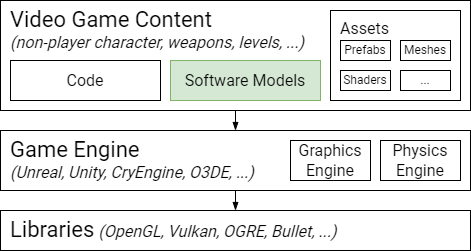
\includegraphics[width=0.45\textwidth]{Figures/ArchitectureLayers.drawio.png}
    \caption{Overview of video game artifacts. Highlighted in green Software Models, where this work focus.}
    \label{fig:architecture}
\end{figure}

\subsection{Case Study: \CaseStudy{}}
\label{subsec:case_study}

The case study that we use to evaluate the work presented here is
performed using the bosses of the video game Kromaia. The game
in Kromaia takes place in a three-dimensional space. Each of the
levels involves a player’s spaceship flying from a starting point to
a target destination reaching the goal before being destroyed. The
level involves exploring floating structures, avoiding asteroids, and
finding items along the route, while protected by basic enemies
that try to damage the player’s spaceship by firing projectiles. If
the player manages to reach the destination, the final boss corresponding
to that level appears and must be defeated in order to
complete the level.

The bosses are specified with the Shooter Definition Model Language
(SDML). SDML is a DSL model for the video game domain.
This DSL follows the main ideas of MDE using models for Software
Engineering. The models are created using SDML and interpreted
at runtime. Specifically, SDML defines aspects that are included
in video game entities: the anatomical structure (including which
parts are used in it, their physical properties, and how they are
connected to each other); the amount and distribution of vulnerable
parts, weapons, and defenses in the structure/body of the character;
and the movement behaviours associated to the whole body or its
parts. This modeling language has concepts such as hulls, links,
weak points, weapons, and AI components. Examples of the models,
the metamodel, and an online visualizer to show the models as
they would be seen in the Kromaia video game can be found at the
following URL: https://svit.usj.es/models22/bl-in-mgse. \todo{Modify link}

The simulations used in this work simulate a duel between a boss and a human player. The simulated player is an algorithm that is able
to act like a human player. It was created by the developers of the
Kromaia video game. We used their algorithm for our approach.
During the simulation, the simulated player faces the boss in order
to destroy the weak points that are available at that moment,
whereas the boss acts according to the anatomy, behaviour, and
attack/defense balance that is included in its model, trying to defeat
the simulated player. In the simulation, both the boss and the
simulated player try to win the match and do not avoid confrontation,
try to prevent draw/tie games, and try to ensure that there
is a winner. The algorithm can fight a boss by applying different
strategies. Hence, the algorithm can be parametrized to define the
fighting strategy. The simulation parameters were provided by the
developers based on the analysis of battles between human players
and bosses.

It is important to clarify that bosses can be built either using
SDML software models or directly with C++. The intuition of the
developers is that they make fewer mistakes and are more efficient
working with the models than with the code, and an experiment
confirmed this [15]. \mar{check if the clarification of models and code is in other part, if not adapt it. The part of the mistakes should not be relevant to our work.}
\section{Our \ApproachName{} Approach} \label{sec:Approach}

This section will explain how our approach make use of evolutionary computation to transplant elements within video games content. Figure~\ref{fig:approach} shows our \ApproachName{} approach that we will explain in detail during this section. We will also make use of a theoretical example of auto-transplantation of content within a simplified version of "bosses" of the video game Kromaia.

\begin{figure}[h]
    \centering
    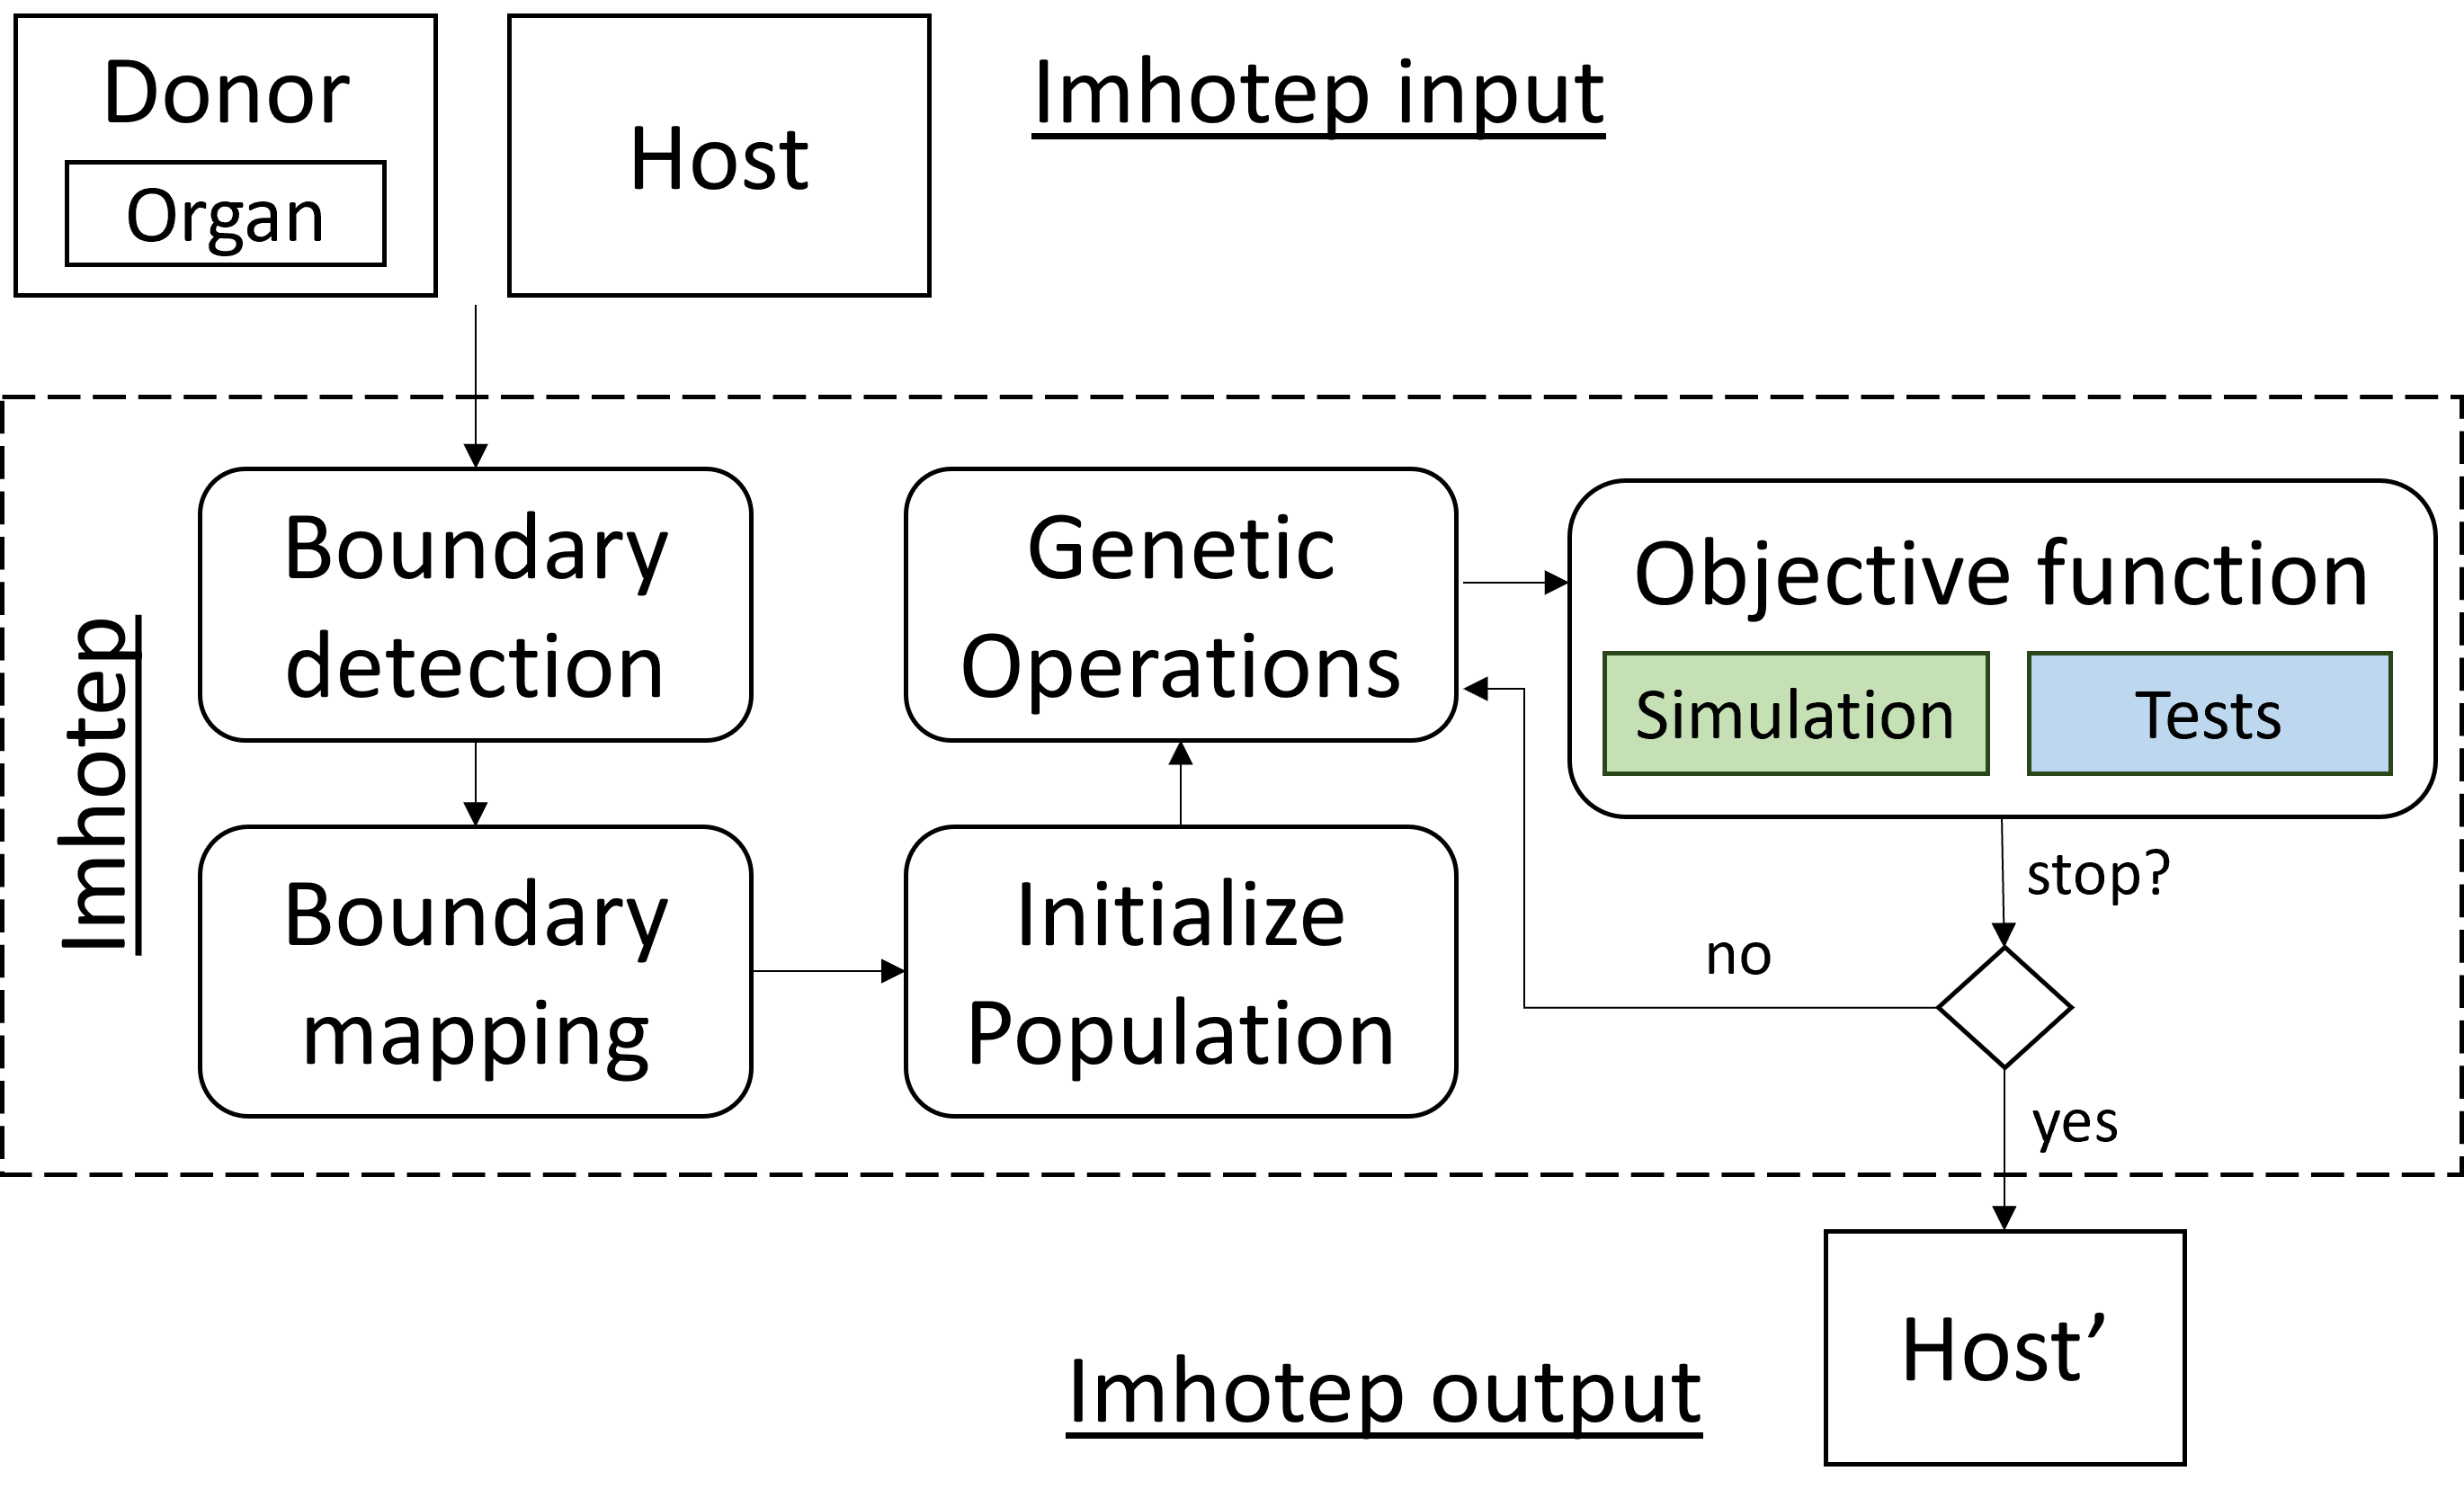
\includegraphics[width=0.45\textwidth]{Figures/overview.png}
    \caption{Overview of Imhotep}
    \label{fig:approach}
\end{figure}


\subsection{Input selection}

The very first step of our approach is the definition of the input. \ApproachName{} requires the developers to define a source model content (donor) with the organ that will be transplanted, and a target model content (host). The models used in \ApproachName{} are models based on SDML as explained in the background section (\ref{subsec:case_study}). The donor and host from the example are different from the donor and host used in the evaluation, but we think they will help to understand the approach. The donor, organs and host used by \ApproachName{}

For the theoretical example we present a simplified version of the metamodel, and its corresponding concrete syntax of the model (Fig.~\ref{fig:metamodel+syntax}) from the video game \CaseStudy{}. In this example we use a graphical representation to help the comprehension of the reader. Notice that the original metamodel does not work with a graphical model representation as it is not a requirement on every metamodel. The type of model will depend on the metamodel and models that developers decide on.

\begin{figure}[h]
    \centering
    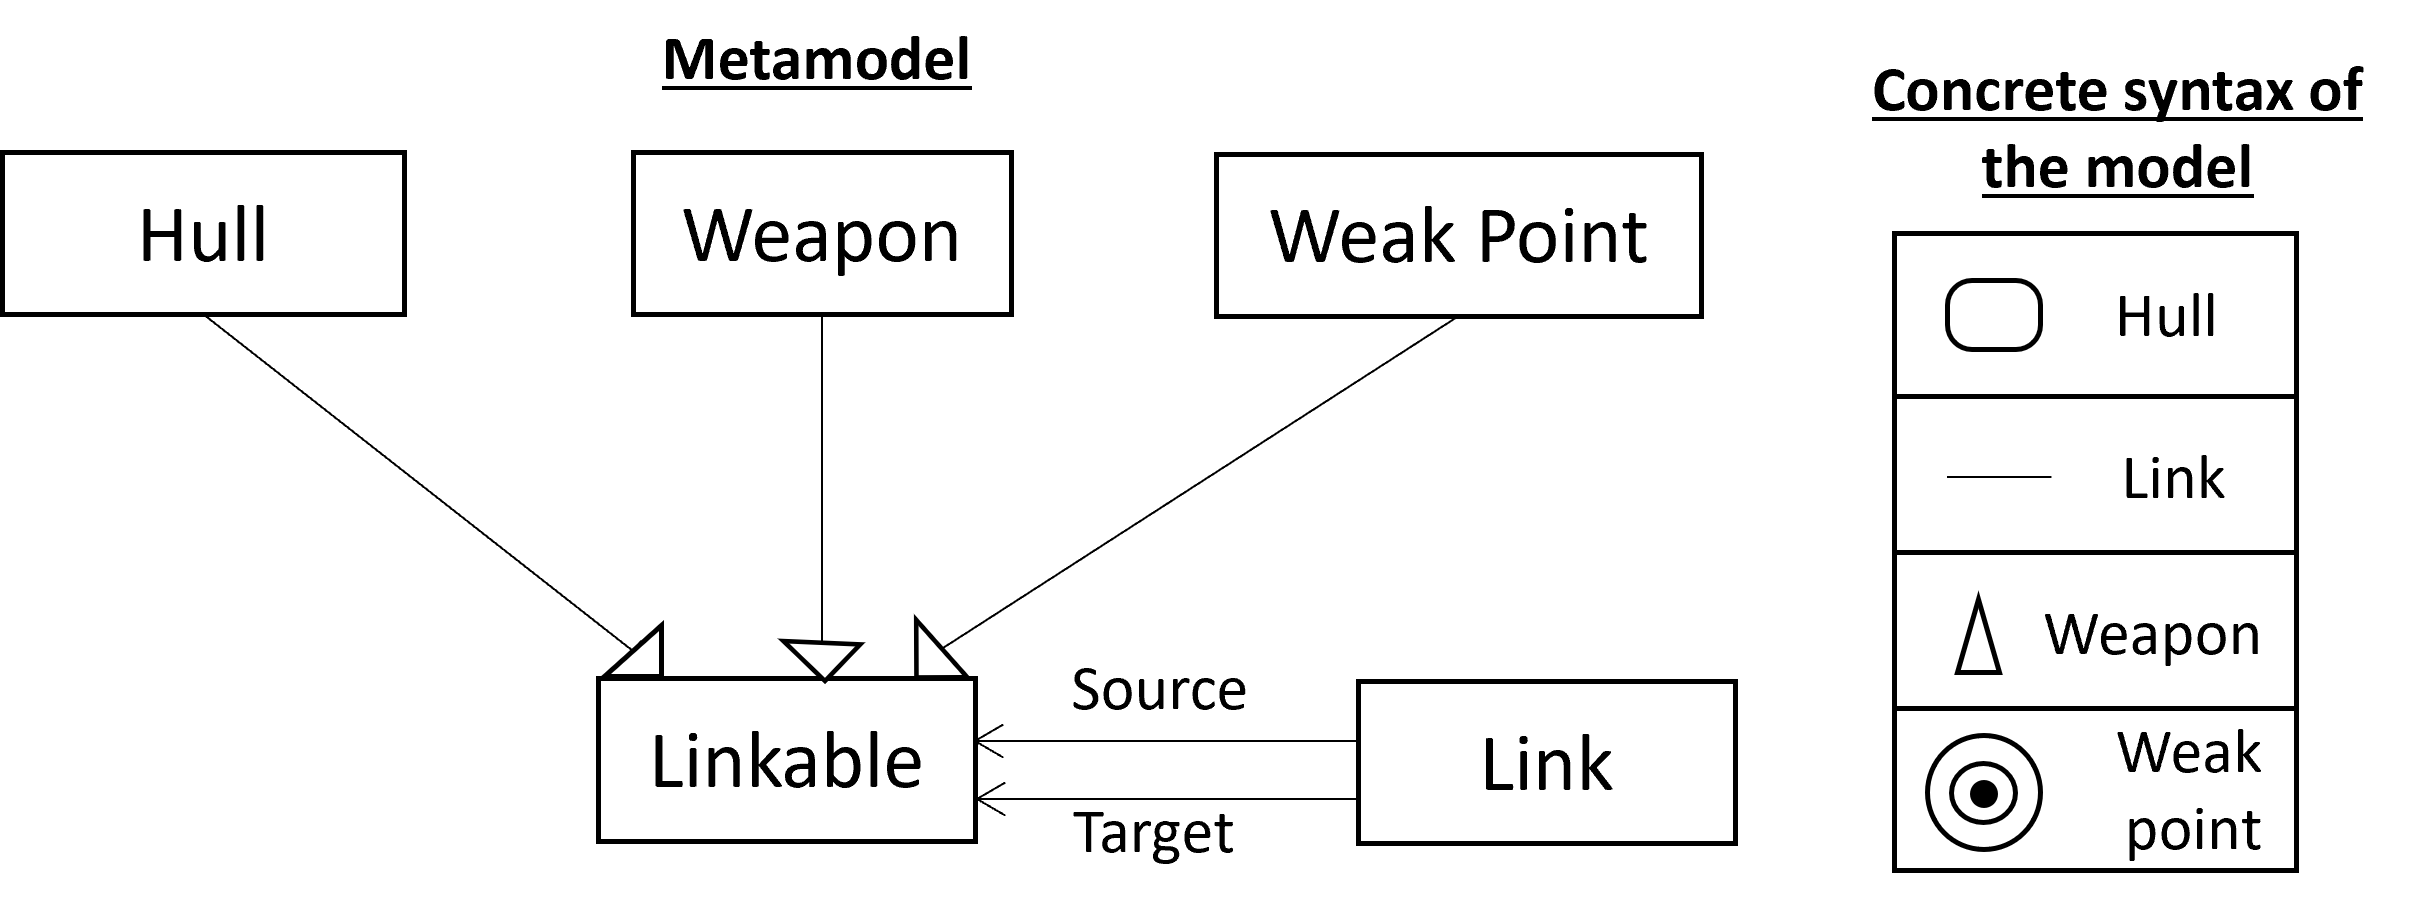
\includegraphics[width=0.45\textwidth]{Figures/metamodel+syntax.png}
    \caption{Simplified metamodel with its corresponding concrete syntax of the model}
    \label{fig:metamodel+syntax}
\end{figure}

Based on the metamodel of our example, we define the inputs as stated. 
First, we define the source donor, that is a simplified version of an original "boss" from \CaseStudy{}, called "Serpent" (Fig.~\ref{fig:donor}). The original model is a SDML model written on a XML file with approximately 1700 lines of code. Figure~\ref{fig:donor} shows the graphical representation of the donor, differentiating each element of the model with a letter from A to S. It also shows in green the elements selected as organ (the elements H, I, J, K, N, O, P, Q).
Secondly, we define the host of our example. To that extent, we have created a regular enemy that could appear on \CaseStudy{} following the metamodel (Fig.~\ref{fig:host}.

\begin{figure}[h]
    \centering
    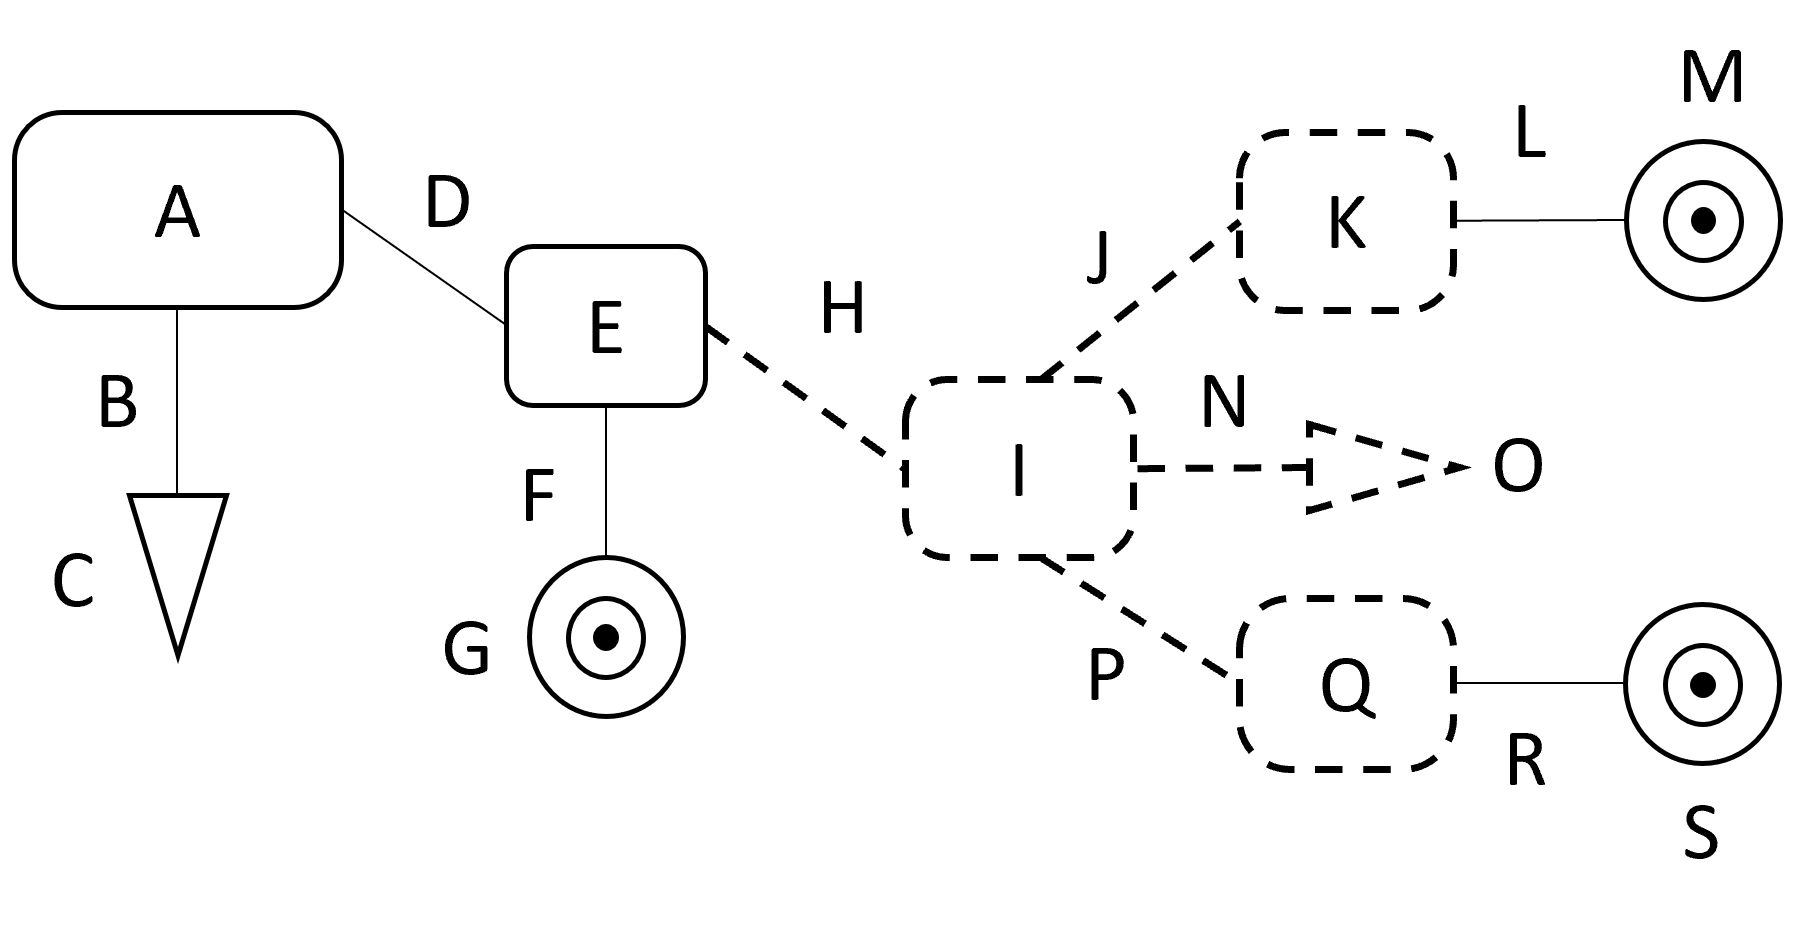
\includegraphics[width=0.45\textwidth]{Figures/donor+organ.png}
    \caption{Donor with organ selection in green. The letters represent each element of the model.}
    \label{fig:donor}
\end{figure}

\begin{figure}[h]
    \centering
    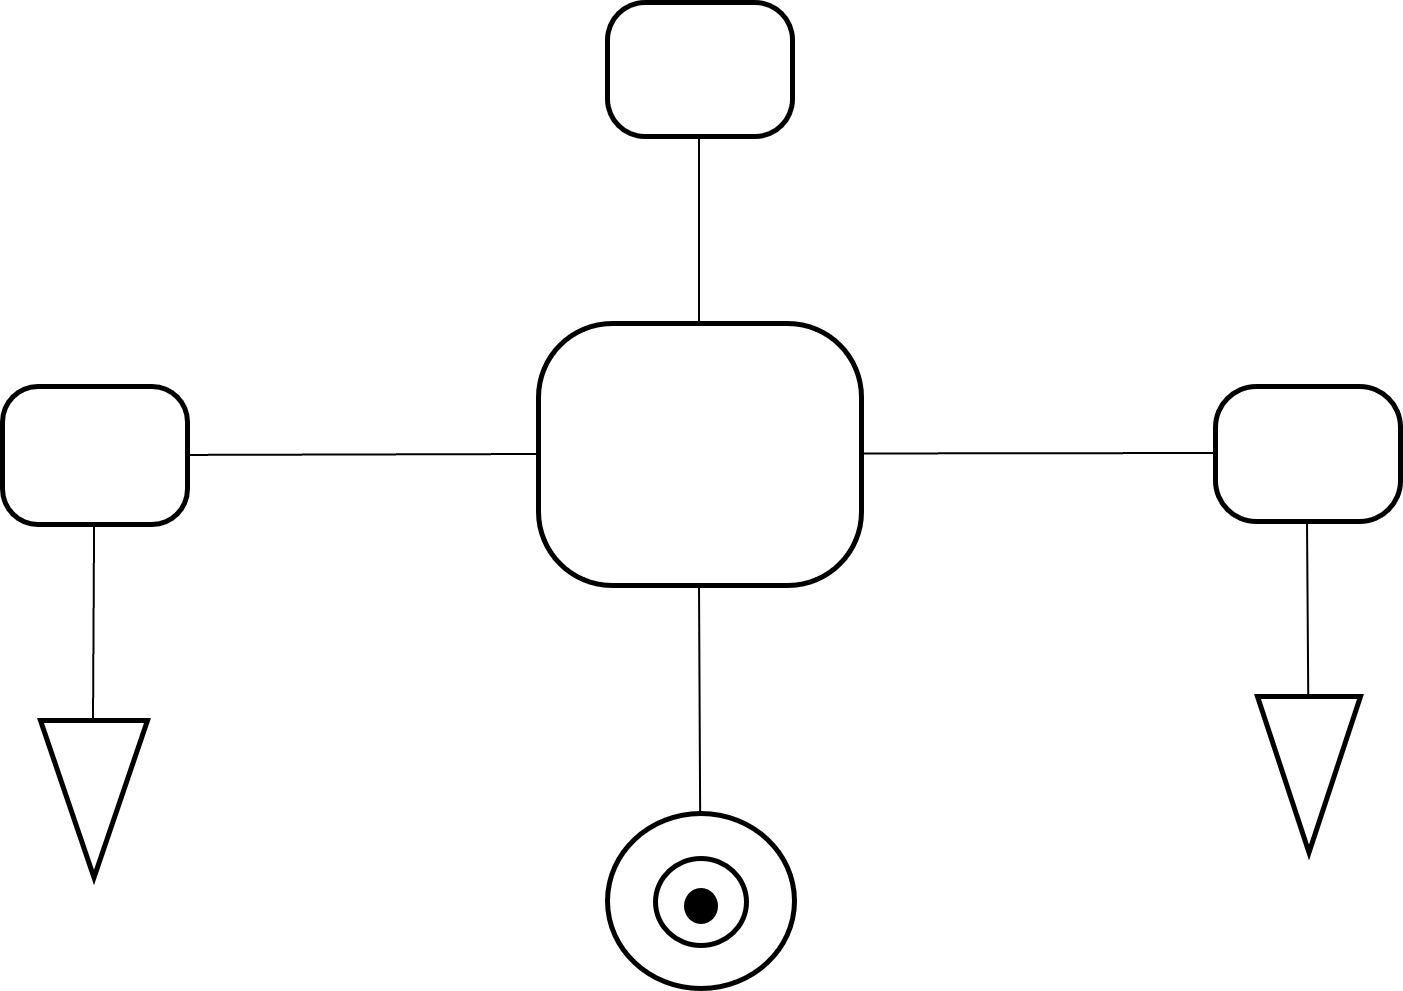
\includegraphics[width=0.3\textwidth]{Figures/host.png}
    \caption{Host}
    \label{fig:host}
\end{figure}

\subsection{Boundary detection}

To transplant an organ into a host we need to find a way to connect them. To do that we will use the boundaries of the organ and the host. A boundary is a connection point on an element capable of connect two elements within a model. The connection is restricted by the rules of the metamodel. \ApproachName{} identifies the boundaries of the selected organ, and all the boundaries of the host before initializing the evolutionary algorithm.

Following on our example the approach will detect the boundaries of the organ, and the host. The boundaries of the organ will be the connection points between donor and host. The elements that connect with the rest of the donor are H, K, and Q. We can then state the boundaries on each element. Figure~\ref{fig:org_bound} shows the donor, the organ, and the boundaries (boundaries are represented by a circle crossed). The boundaries of the organ will be; b11 for the H element; b16 for the K element, and b25 for the Q element.

\begin{figure}[h]
    \centering
    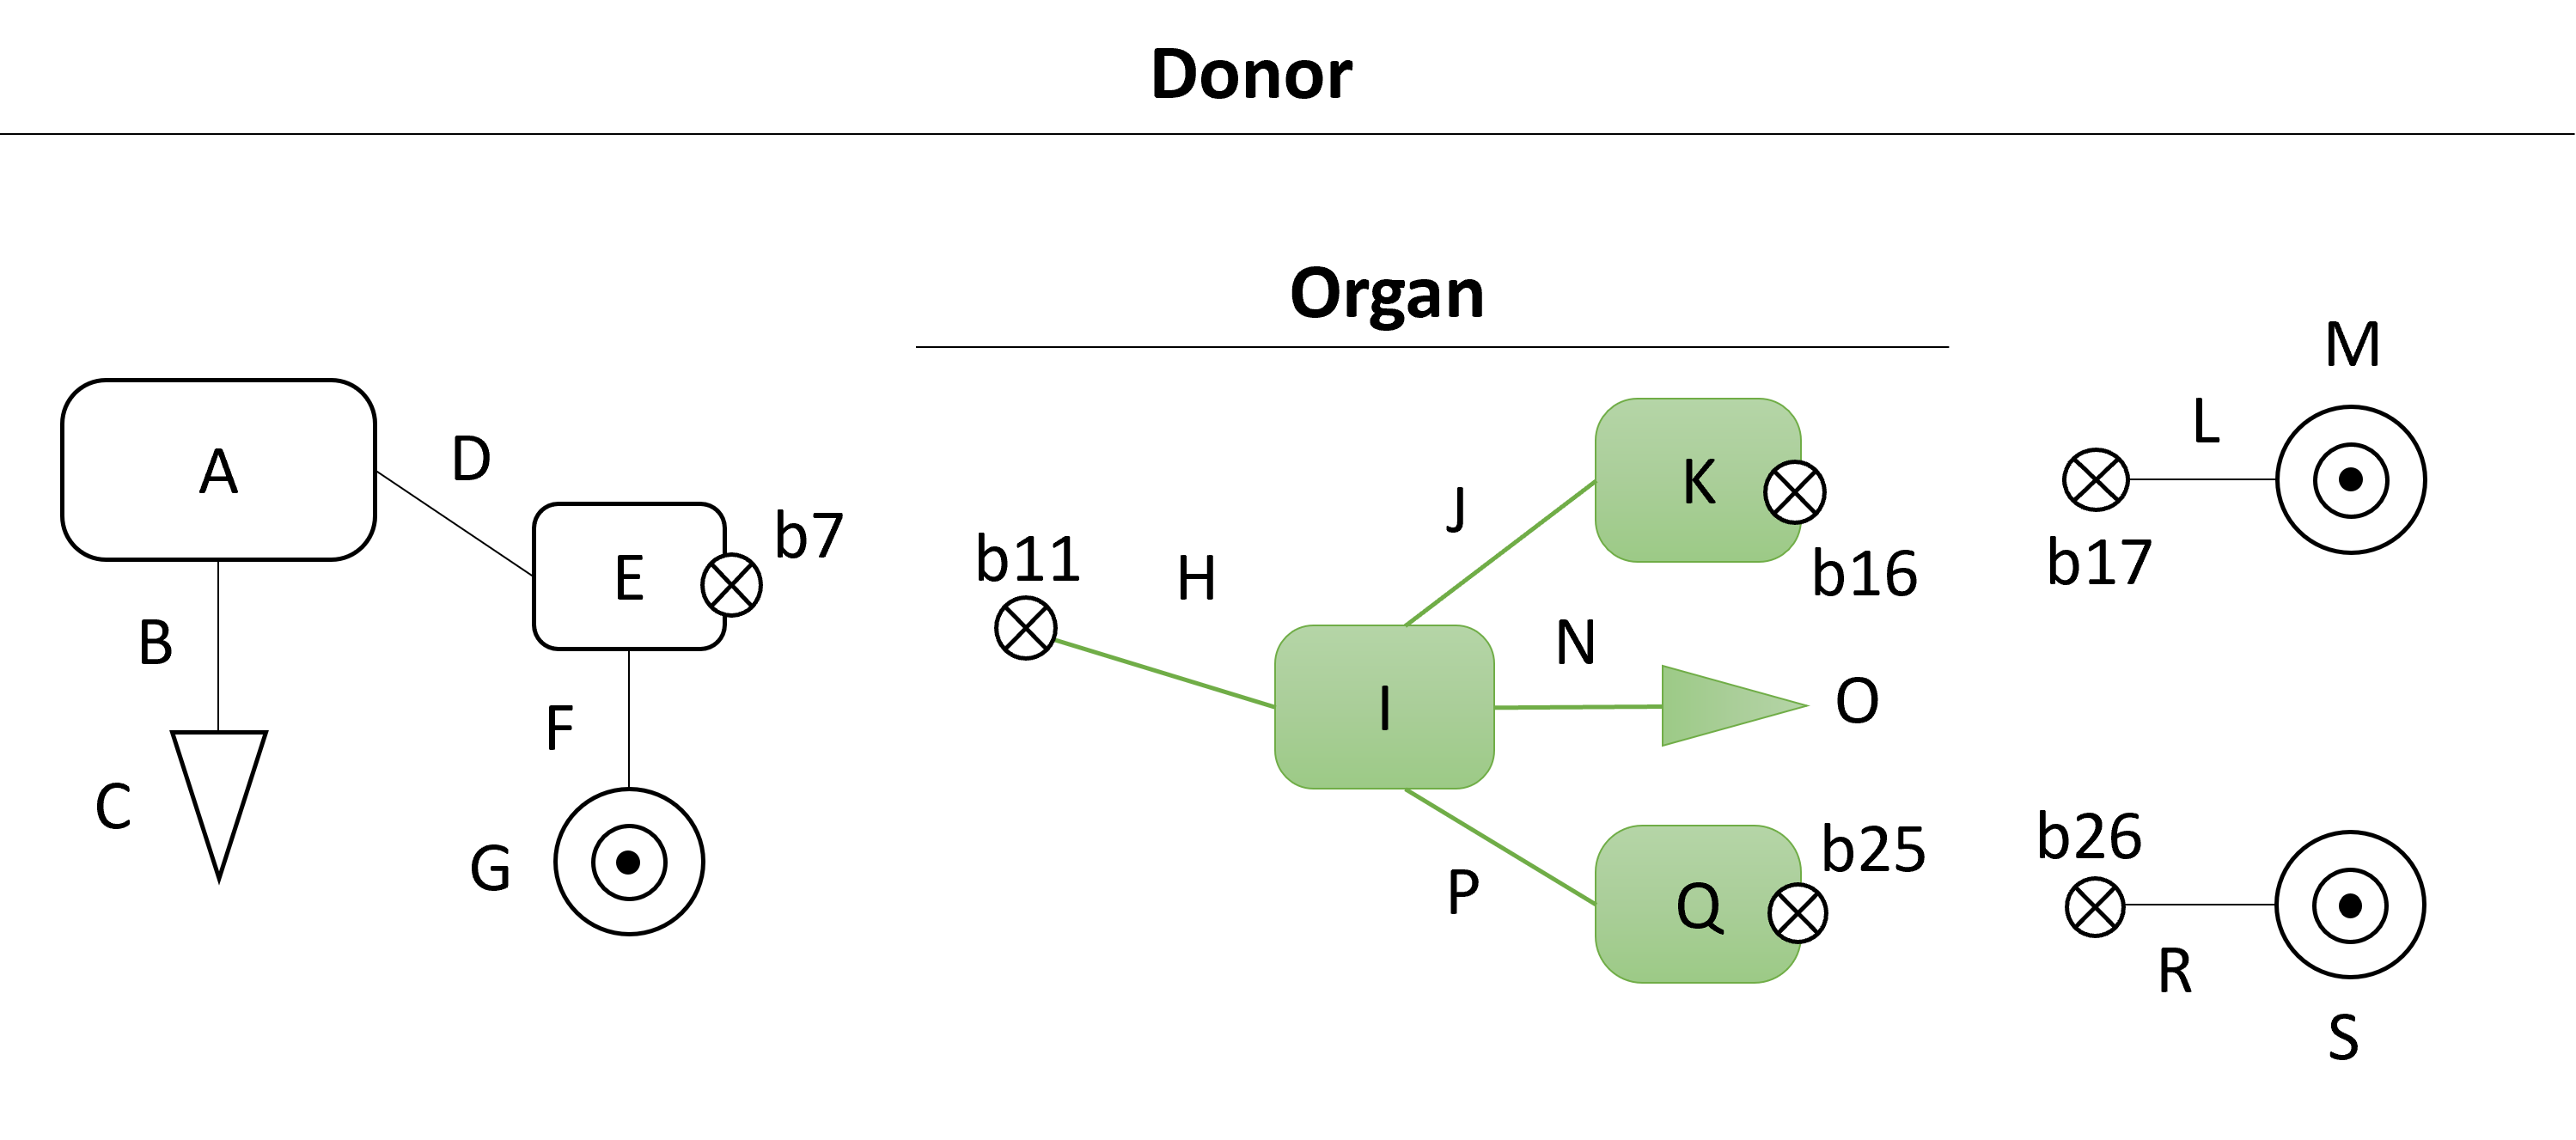
\includegraphics[width=0.45\textwidth]{Figures/donor+organ_boundaries.png}
    \caption{Definition of organ boundaries. The boundary is represented by a circle crossed.}
    \label{fig:org_bound}
\end{figure}

On the other hand, the boundaries of the host will be all the points where its elements connect. Figure~\ref{fig:host_bound} shows all the boundaries of the host of the example. The host has a total of 19 boundaries identified by a tag from ba to bs.

\begin{figure}[h]
    \centering
    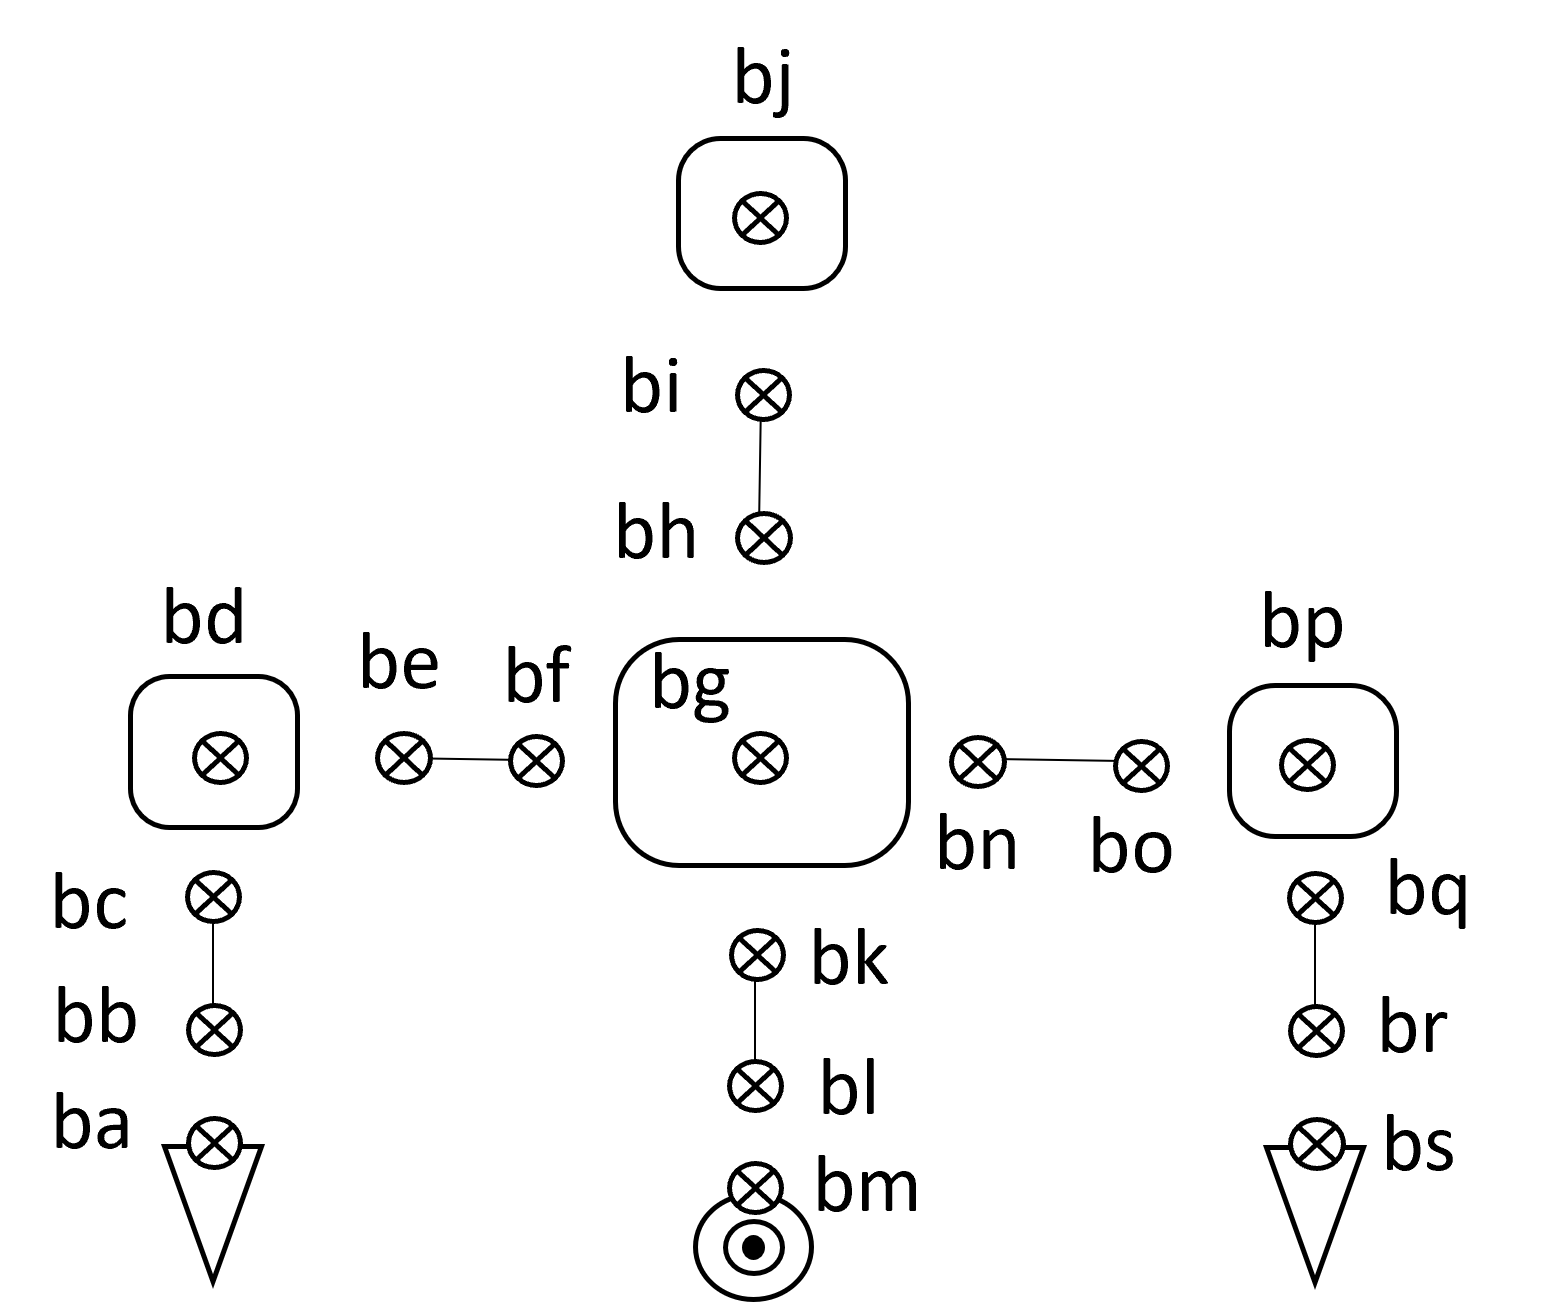
\includegraphics[width=0.45\textwidth]{Figures/host_boundaries.png}
    \caption{Definition of host boundaries. The boundary is represented by a circle crosed.}
    \label{fig:host_bound}
\end{figure}

\subsection{Boundaries mapping}

In the boundary mapping step, \ApproachName{} determine the relation between the boundaries of the organ and the host. From each boundary in the organ we map the all possible connections that could have with boundaries of the host, including the possibility of not connecting the boundary to the host boundaries (Table.~\ref{tab:boundaries}. 

Table~\ref{tab:boundaries} map the compatible boundary connections between organ and host. The boundary b11 is a boundary from a "Link" from the model and according to the metamodel it can connect to any "Hull", "Weapon", "Weak Point" or remain unconnected. The boundaries b16 and b25 are both "Hulls" and they can connect with any "Link" or remain unconnected.

\begin{table}[h]
\centering
\begin{tabular}{|c|ll|}
\hline
{\color[HTML]{000000} Organ boundary}                                     & \multicolumn{2}{c|}{{\color[HTML]{000000} \begin{tabular}[c]{@{}c@{}}Host \\      boundaries\end{tabular}}} \\ \hline
                                                                          & \multicolumn{1}{c|}{ba}                         & \multicolumn{1}{c|}{bm}                                   \\ \cline{2-3} 
                                                                          & \multicolumn{1}{c|}{bd}                         & \multicolumn{1}{c|}{bp}                                   \\ \cline{2-3} 
                                                                          & \multicolumn{1}{c|}{bg}                         & \multicolumn{1}{c|}{bs}                                   \\ \cline{2-3} 
\multirow{-4}{*}{b11}                                                     & \multicolumn{1}{c|}{bj}                         & \multicolumn{1}{c|}{Not connected}                        \\ \hline
                                                                          & \multicolumn{1}{c|}{bb}                         & \multicolumn{1}{c|}{bc}            \\ \cline{2-3} 
                                                                          & \multicolumn{1}{c|}{be}                         & \multicolumn{1}{c|}{bf}                     \\ \cline{2-3} 
                                                                          & \multicolumn{1}{c|}{bh}                         & \multicolumn{1}{c|}{bi}                                                        \\ \cline{2-3} 
                                                                          & \multicolumn{1}{c|}{bk}                         & \multicolumn{1}{c|}{bl}                                                        \\ \cline{2-3} 
                                                                          & \multicolumn{1}{c|}{bn}                         & \multicolumn{1}{c|}{bo}                                                        \\ \cline{2-3} 
\multirow{-6}{*}{\begin{tabular}[c]{@{}c@{}}b16\\    \\ b25\end{tabular}} & \multicolumn{2}{c|}{Not connected}                                                                          \\ \hline
\end{tabular}
\caption{Mapping  of compatible boundaries between organ and host}
\label{tab:boundaries}
\end{table}

\subsection{Encoding}

Te adjunto el encoding que había originalmente, al que habría que añadir una fila nueva "transplant root hull index": en ella todo son guiones "-" (representa -1), salvo en los cascos que están ahí porque han sido implantados. En todos ellos aparecerá un número/carácter que representa el índice del casco del receptor por el que el empalme se ha realizado, mediante link. En el otro archivo que te paso, el gusano (64 cascos originalmente) tiene trasplantado un brazo que tiene 13 cascos. El primero de esos trece está unido al número 14 del gusano (en la fila de links, el casco 65, el primero correspondiente al contenido trasplantado, tiene una "e"(14). Ésa "e" es la que luego ves en la última fila, en las columnas correspondientes al contenido trasplantado.

\subsection{Genetic Operators}

Imhotep has three genetic operations (selection, crossover, and mutation) to generate new individuals. To select the individuals we use the ranking selection, which ranks the population by the objective function and takes the top 10\% of the individuals in the current population. The size of the population is limited to 100, i.e the selection will take 10 individuals to apply crossover between them.

\todo{how crossover work?}

The new individual then have a probability of 1/150 to mutate any value of the encoding. The probability is based on the size of the encoding of an individual which is 150 in our approach.

After all the operations have been applied, the new set of individuals are evaluated by the objective function and added to the population. The last individuals by ranking in the population are discarded to maintain the size of the population on 100. 

Figure.~\ref{fig:candidates} shows handmade new individuals that could results from our example.

\begin{figure}[h]
    \centering
    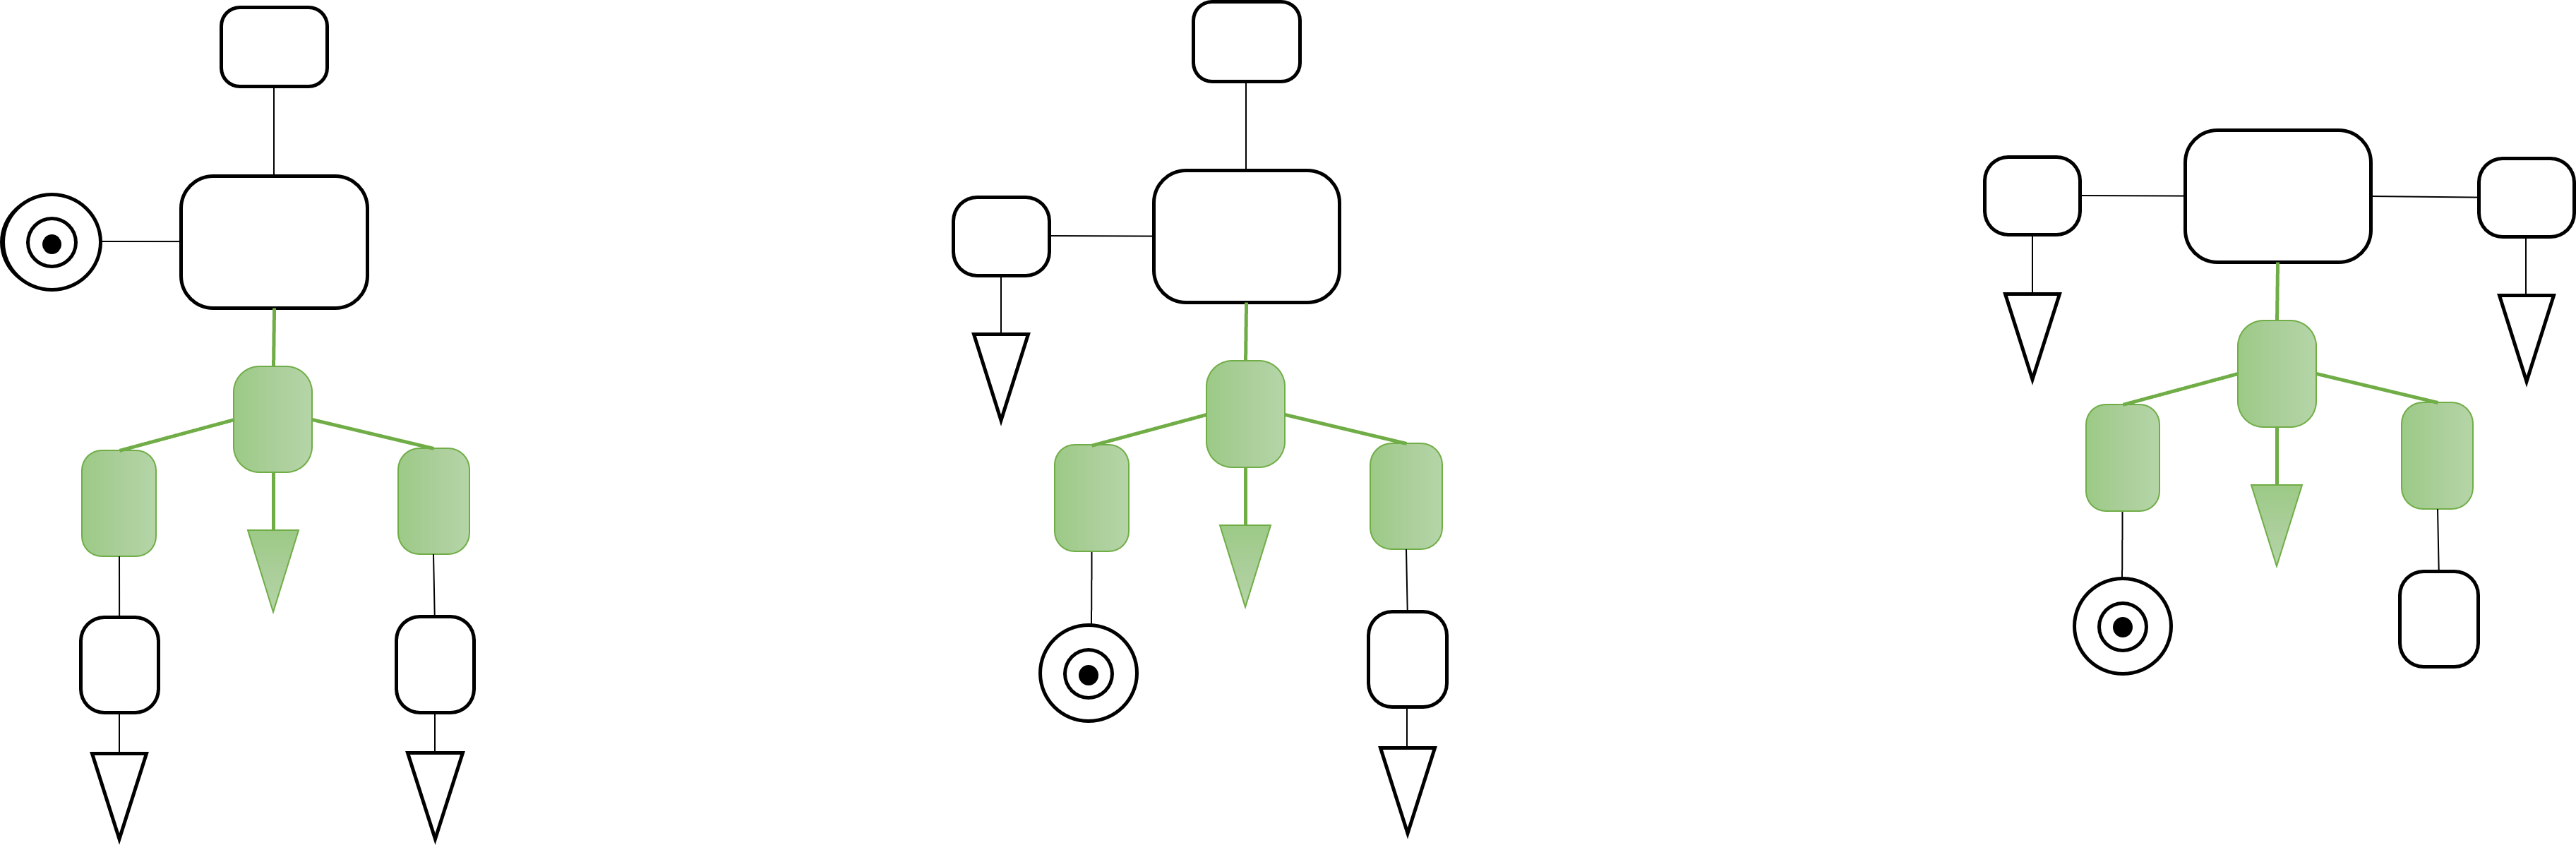
\includegraphics[width=0.45\textwidth]{Figures/candidates.png}
    \caption{Population individuals to be evaluated by the objective function}
    \label{fig:candidates}
\end{figure}

\subsection{Objective function}

The objective function in \ApproachName{} assess the quality of each individual as a model. First, as done in previous work of that use the case study \CaseStudy{}~\cite{blasco2021evolutionary}, the models pass through a validation process followed by a quantitative measurement. In our work we assess quantitatively the objective function by two means; Test-based and Simulation-based objective functions. We use two different objective functions due to the differences in the the state-of-the-art of software transplantation and PCG. The state-of-the-art in software transplantation mainly work with Test-based objective function, while the state-of-the-art in NPCs PCG work with Simulation-based objective function.

The validation step before the Test-based or Simulation objective function is a requirement that \CaseStudy{} integrates in the game to avoid models with inconsistent data. The validity of the models is performed by a run-time interpreter that is part of the game. When the model is stated as non-valid the value of the objective function will be 0.0.

The models that passes the validation process will then be assess by Test-based and Simulation-based objective function.
For the Test-based objective function we ask the developers to provide the set of tests that they consider relevant to our work. The developers from \CaseStudy{} provided us a total of 243 test selected under they domain knowledge. The objective value will be retrieved when each individual pass through the 243 tests normalized in a scale of [0, 1] written this limitation. An individual which pass the 243 tests will obtain 1.0, and on the contrary if it does not pass any test will obtain 0.0.

On the other hand, the Simulation-based objective function as in Blasco \etal~\cite{blasco2021evolutionary} simulates an in game battle between the boss and a player. The information retrieved from the simulation is the data that the developers regard as relevant, using their domain knowledge. Hence, our approach takes into account the percentage of simulated player victories ($F_{Victory}$) and the percentage of simulated player health left once the player wins a duel ($F_{Health}$).
The calculation of $F_{Victory}$ and $F_{Health}$ is performed in the same
way as Blasco \etal~\cite{blasco2021evolutionary}:

$F_{Victory}$ is calculated as the difference between the number of human player victories ($V_{P}$) and the optimal number of victories (33\%, according to the developers of \CaseStudy{} and their criteria) ($V_{Optimal}$):
\begin{equation}
F_{Victory} = 1 -\frac{\mid V_{Optimal} - V_{P} \mid}{ V_{Optimal}}
\end{equation}

$F_{Health}$, which refers to completed duels that end in human player victories, is the average difference between the human player's health percentage once the duel is over ($\Theta_{P}$) and the optimal health level that the player should have at that point ($\Theta_{Optimal}$, 20\%, according to the developers):
\begin{equation}
F_{Health} = 1 - \frac{\sum\limits_{d=1}^{V_{P}}\frac{\mid \Theta_{Optimal} - \Theta_{P} \mid}{ \Theta_{Optimal}}}{V_{P}}
\end{equation}

$F_{Overall}$ is an average fitness value for a boss model that includes the fitness criteria described above. In the end, $F_{Overall}$ is a value in [0, 1] that is used to assess a boss model when our \ApproachName{} approach is applied to the \CaseStudy{} case study.

\begin{equation}
F_{Overall} = min( Validity, \frac{\sum\limits_{i=1}^{N}F_{i}}{N} )
\end{equation}

\section{Evaluation} \label{sec:Evaluation}

In this section we explain how we evaluate the feasibility of automated transplantation in video games through our \ApproachName{} approach. Our experiment compares \ApproachName{} with the two different objective functions, Test-based and Simulation-based, and a PCG baseline. 

The PCG baseline that we use is... \todo{explain the baseline}

We transplant on 5 different host, original bosses from the video game \CaseStudy{}. We have 129 donors, that are elements from the scenario of the game, called "Totems". We obtain a total of 645 new host' from Simulation-based and 645 new host' from Test-based. \todo{for the baseline we force 129 repetitions per initial boss, so we obtain 645 new host as well}

The execution time for each transplantation is 2 minutes and 30 seconds.

We run the experiments in two laptops with the following specifications; Intel Core i7-8750H, 16GB, 2.2GHz; and  2x Intel(R) Xeon(R) CPU X5660, 64GB, 2.80GHz.

We evaluate each host' with the following quality measures:

\subsection{Quality measurements}
\label{subsec:Measurements}

In a recent research done by Browne et al., the experimentation with game users showed that the following criteria stand out as being the most important: Completion, Duration, Uncertainty, Killer Moves, Permanence, and Lead Change \cite{browne2010evolutionary}. Our evaluation measures these criteria with values in the interval [0,1].

{\bf Completion (Viability):} A game against a boss unit should end with more conclusions (victories for either the player or the boss) than draws/ties. The criterion $Q_{Completion}$ calculates a ratio of conclusions over total duel count:
\begin{equation}
Q_{Completion} = \frac{Conclusions}{Duels}
\end{equation}

{\bf Duration (Viability):} The duration of duels between players and boss units is expected to be around a certain optimal value. For the video game case study, through tests and questionnaires with players, the developers determined that concentration and engagement for an average boss reach their peak at approximately 10 minutes ($T_{Optimal}$), whereas the maximum accepted time was estimated to be 20 minutes ($2*T_{Optimal}$). Significant deviations from that reference value are good design-flaw indicators: short games are probably too easy; and duels that go on a lot longer than expected tend to make players lose interest. The criterion $Q_{Duration}$ is a measure of the average difference between the duration of each duel ($T_{d}$) and the desired, optimal duration ($T_{Optimal}$):
\begin{equation}
Q_{Duration} =  1 - \frac{\sum\limits_{d=1}^{Duels}\frac{\mid T_{Optimal} - T_{d} \mid}{T_{Optimal}}}{Duels} 
\end{equation}


 {\bf Uncertainty (Quality):} In order to keep players engaged with a duel, neither the player nor the boss unit should get extremely close to victory or defeat too early before the duel is settled, with ($T_{d}$) being its duration. Therefore, a duel is considered to be more uncertain the longer the time until the player's or the boss unit's health levels reach a dangerous/critical status ($P_{d}$ and $B_{d}$, respectively). For each duel, $Q_{Uncertainty}$ measures the average deviation between the time at which it is detected that one of the contenders is on the verge of defeat and the time corresponding to the duration of the duel.
\begin{equation}
Q_{Uncertainty} =  1 - \frac{\sum\limits_{d=1}^{Duels}\frac{T_{d} - min\left ( P_{d}, B_{d} \right )}{T_{d}}}{Duels} 
\end{equation}

{\bf Killer Moves:}   $Q_{KMoves}$ measures the proportion of killer moves by any contender ($K$), taking into account the moves that are considered to be remarkable highlights ($H$) but that are less important than killer moves. In the video game case study, the developers considered that a highlight move happens when either the boss unit or the player experiences a decrease in health; killer moves are those that make the difference in health between the contenders reach 30\%.
\begin{equation}
Q_{KMoves} =  1 - \frac{\sum\limits_{d=1}^{Duels}\frac{K_{d}}{H_{d}}}{Duels} 
\end{equation}

{\bf Permanence:} Duels with a high permanence value are games in which the advantages given by significant actions or moves by one of the contenders are unlikely to be immediately reverted by the opponent in terms of dominance. In the video game case study, the developers considered every highlight move and killer move to be meaningful actions, with recovery moves ($R$) being those that quickly cancelled the advantages given by other previous killer or highlight moves. The criterion $Q_{Permanence}$ is measured as follows:
\begin{equation}
Q_{Permanence} =  1 - \frac{\sum\limits_{d=1}^{Duels}\frac{R_{d}}{H_{d}+K_{d}}}{Duels} 
\end{equation}

{\bf Lead Change:} The lack of lead changes indicates low dramatic value. In the video game case study, the lead is determined at any given moment by considering the contender with the highest health level. This criterion is measured taking into account those highlight or killer moves that cause the lead to change ($L$) during the course of a duel:
\begin{equation}
Q_{LChange} = \frac{\sum\limits_{d=1}^{Duels}\frac{L_{d}}{H_{d}+K_{d}}}{Duels} 
\end{equation}

$Q_{Overall}$ calculates an average quality value for a model, including all of the quality criterion studied:
\begin{equation}
Q_{Overall} = \frac{\sum\limits_{i=1}^{N}Q_{i}}{N}
\end{equation}
\section{Results}
\label{sec:Results}

\begin{figure*}
    \centering
    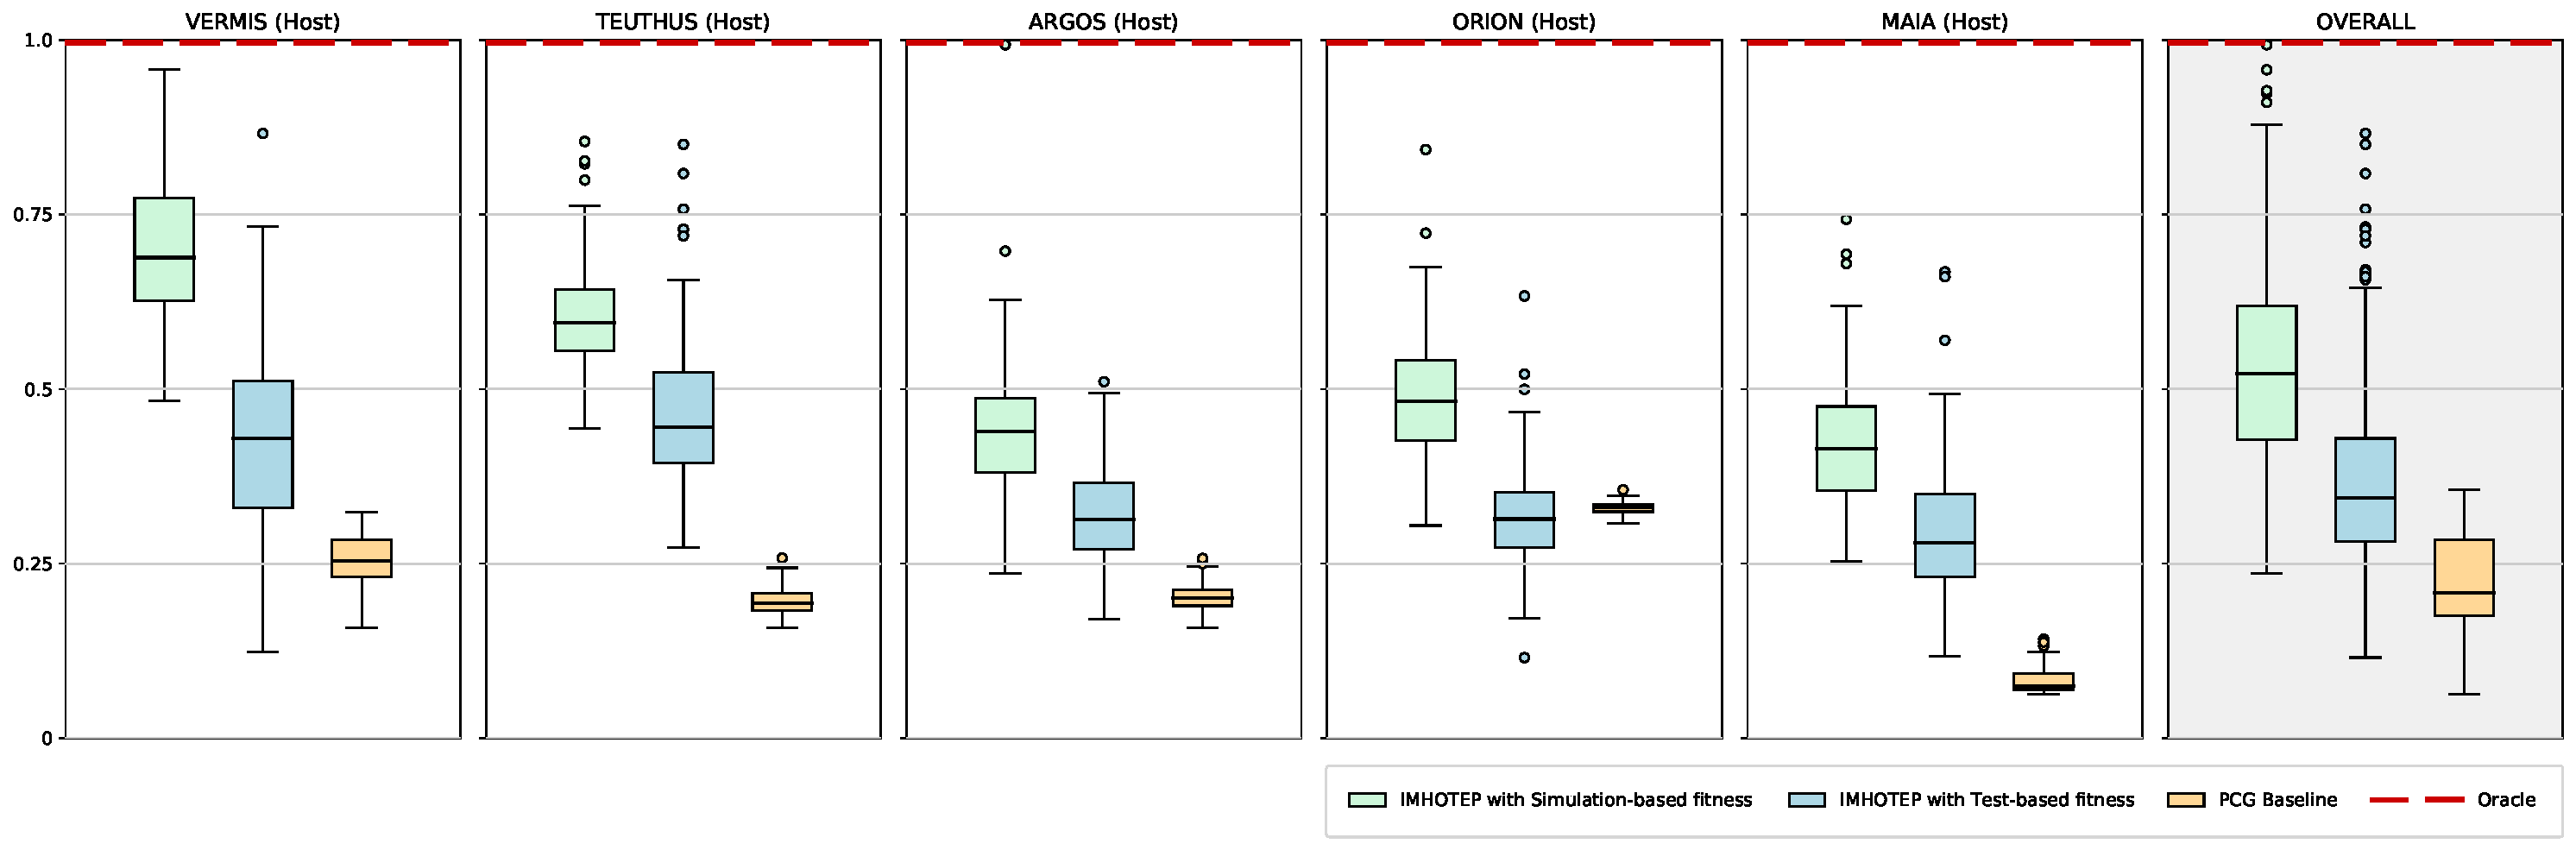
\includegraphics[width=\textwidth]{Figures/Imhotep_with_legend_and_oracle_average-v4.pdf}
    \caption{Results}
    \label{fig:results}
\end{figure*}

Figure \ref{fig:results} shows the results of the evaluation execution of our approach when using the two objective functions (Simulation-Based and Test-Based) from \ApproachName{} and the PCG Baseline. The executions are grouped by each host (boss of \CaseStudy{}) that has been used in our experiment (Vermis, Teuthus, Argos, Orion, and Maia). The last column, with shaded background, shows the average of all of the host for each objective funtion and the baseline. In addition, the oracle indicates the value obtained by the human-generated final boss models that were obtained from the \CaseStudy{}. 

Each boxplot is generated from the results of each host' obtained from the transplantation of each of the 5 hosts with each of the 129 organs. Therefore, each boxplot represents 645 values of a specific host-organ transplantation in a final boss model. Figure \ref{fig:results} shows in each column how the quality values obtained for each of the three strategies studied in our evaluation differ from the values for the models generated by the developers, which are represented by the horizontal red dashed lines that cross each host column. The boxplots that are closer to the horizontal lines are more similar in quality to the models produced by the developers. Additionally, the use of boxplots allows for the representation of the different results for the strategies used.

\todo{Analysis of the results. Simulation has the best results, test also better than baseline...}
\section{Discussion}
\label{sec:Discussion}
\section{Threats to Validity}
\label{sec:Threats}
\section{Conclusion}
\label{sec:Conclusion}


\bibliographystyle{IEEEtran}
\bibliography{references}

\end{document}
